\section{Problem Formulation}
\label{sec_problem_formulation}
In this section, we shows how we formalize the problem of determining the optimal number, placement and distribution of charging station.
\begin{definition}
\label{def_optimal}
\textbf{Optional Distribution:}
Suppose area $a$ is the target area and its graph is $G_{a}(Po(a),\theta(a))$,
the Optional Distribution for $a$ is the solution $\varsigma(a)$ that can meet conditions mentioned in Definition~\ref{def_reachability} and make $a$ is reachable with minimal cost.
\end{definition}
We suppose $X=[x_0, x_1, ......,x_i,......,x_n]$ is a vector, $x_i$ represents the decision of site $i$,
and the value of $x_i$ is defined as:
\begin{equation}
\label{equ_decision_x_i}
x_i =\left\{
\begin{aligned}
& 0 \quad \text{the site $i$ is not used}\\
& 1 \quad \text{the site $i$ is used}\\
\end{aligned}
\right.
\end{equation}
Because we assume the task of optimization belongs to Optimization Layer (the second layer) in Section~\ref{sec_system_architecture},
the input of this problem is the set of potential sites calculated by Selection Layer (the first layer) in our two-layer process architecture.

Suppose the cost of constructing charging station in site $i$ is $c_i$,
then, the total cost of the a solution $\varsigma(a)$ in area $a$ is $Cost_{\varsigma(a)}$,
\begin{equation}
\label{equ_cost}
Cost_{\varsigma(a)} = \sum_{i=0}^{n}x_i \times c_i
\end{equation}
We regard Equation~\ref{equ_cost} as the objective function need to minimize.
After the formulation of the objective function,
we also need to formulate those three conditions mentioned in Definition~\ref{def_reachability}.
\subsection{Condition Formulation}
Because Condition~\ref{con_reach_1} is contained in Condition~\ref{con_reach_3}.
We do not demonstrate it in detail here.

In order to formulate Condition~\ref{con_reach_2} more clearly,
we introduce $Set^{\alpha{R}}(i)$.
For each $i \in Po(a)$
\begin{equation}
Set^{\alpha{R}}(i)=\{j \in Po(a) | d(i,j) \leqslant \alpha{R} \}
\end{equation}
Then, the Condition~\ref{con_reach_2} is equivalent to the equation below,
\begin{equation}
\label{equ_condition_2}
\sum_{j \in Set^{\alpha{R}(i)}} Cap(j) \times x_j \geqslant Demand(i)
\end{equation}

For Condition~\ref{con_reach_3},
it is hard to be formulated directly and we refer to the idea in the work~\cite{lam2013electric}.
We firstly need to generate a graph $G_{a}^{'}({Po}^{'}(a),{\theta}^{'}(a))$ of area $a$,
Specially, ${Po}^{'}(a)$ is set to $Po(a)$ and ${\theta}^{'}(a)$ is defined as:
\begin{equation}
\label{equ_G'}
{\theta}^{'}(a) =\{(i,j) | i,j \in Po(a), d(i,j) \leqslant R, i \neq j \}
\end{equation}
Figure~\ref{fig_graph_example} illustrates an example with $R = 6$ and a 6-node graph,
with the Equation~\ref{equ_G'}, we can generate $G^{'}$ from $G$.
the number on a edge indicates the distance between the nodes on the two ends,
and the number in the circle is the id of the node.
In other words, those nodes i in $G$ with $x_i = 1$ constitute the corresponding induced subgraph~\cite{Induced_Subgraph} $G{'}_{sub}$ of $G^{'}$.
Therefore, we consider that Condition~\ref{con_reach_3} is equivalent to existing \textbf{induced subgraph connected},
and we can use $G^{'}$ to define the problem instead of $G$.
\begin{figure}[!t]
\centering
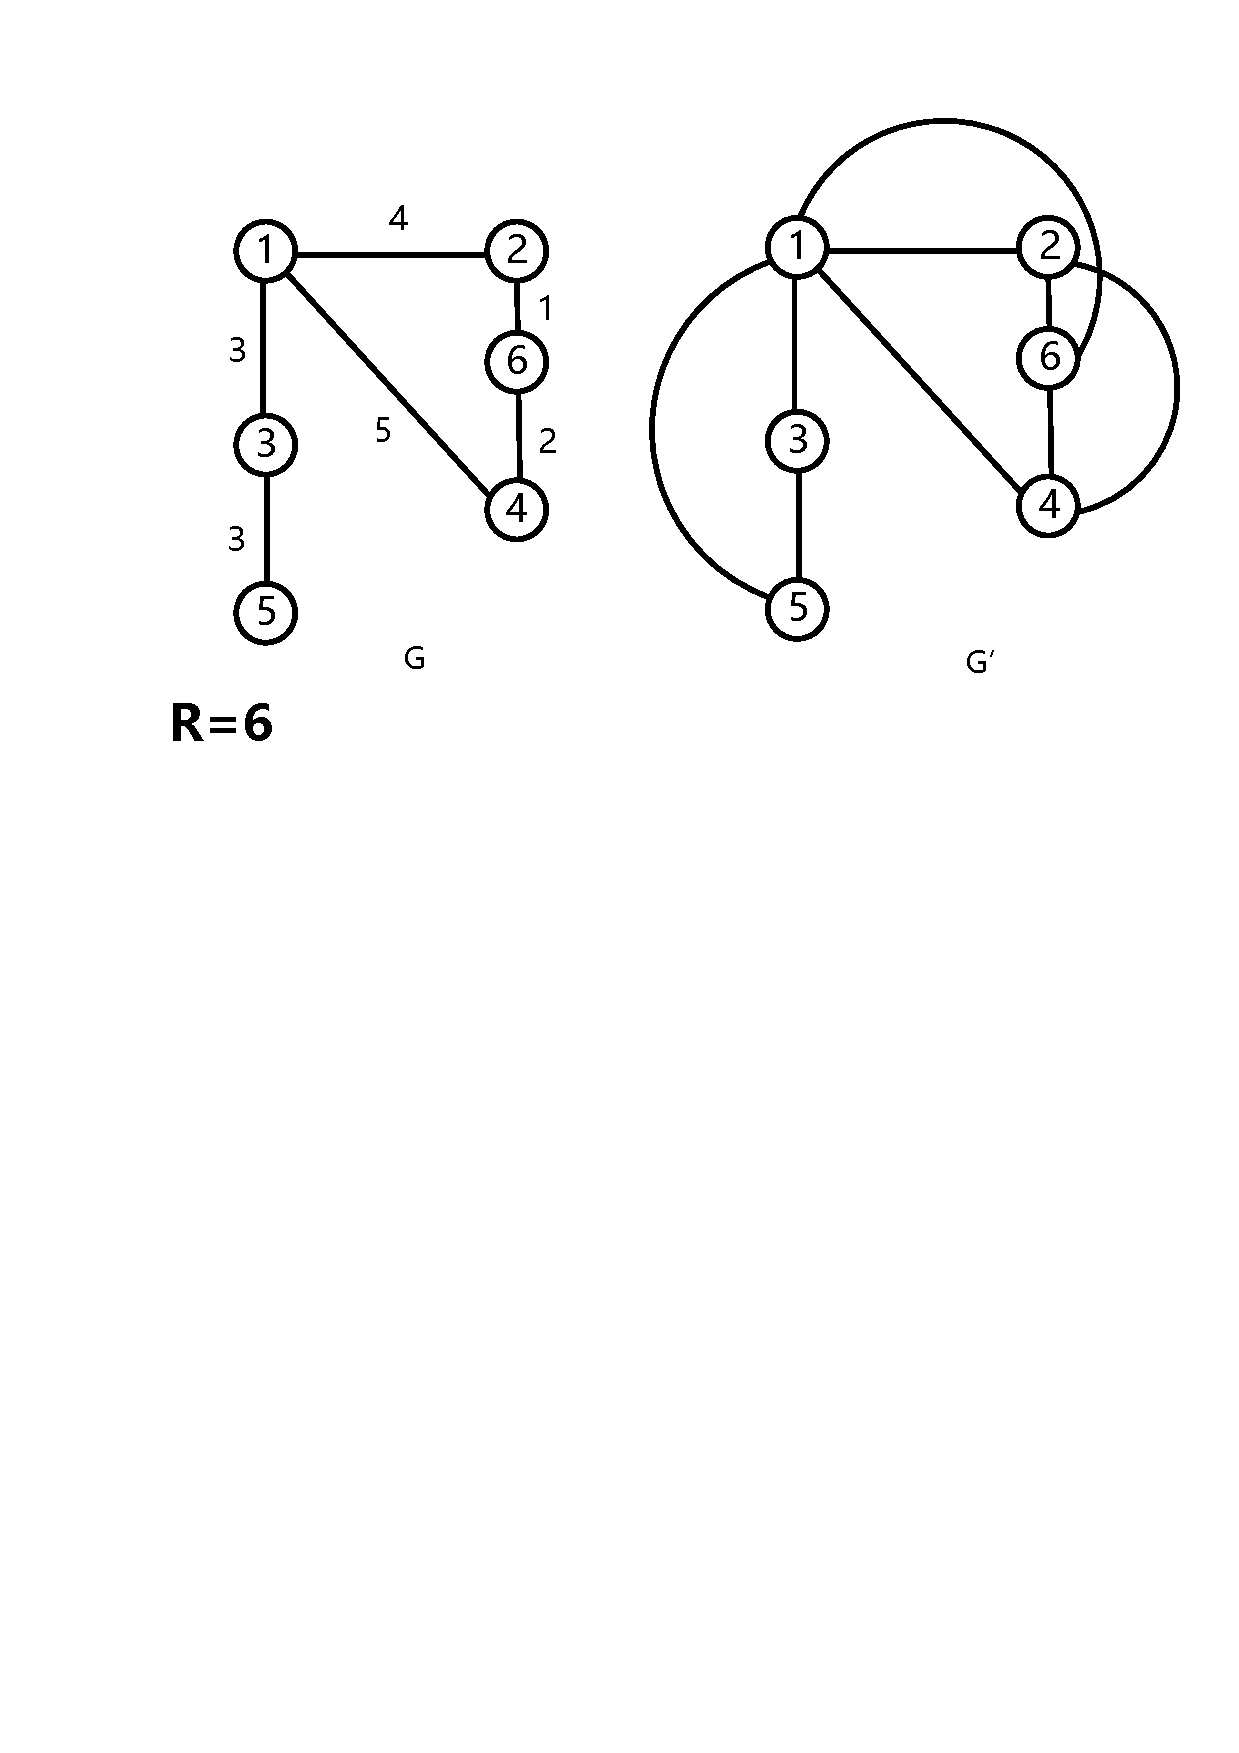
\includegraphics[width=3.5in]{graph_example.pdf}
%\vspace{-0.1in}
\caption{A 6-node Example of $G_{a}(Po(a),\theta(a)) \rightarrow G_{a}^{'}({Po}^{'}(a),{\theta}^{'}(a))$ .}
\label{fig_graph_example}
%\vspace{-0.2in}
\end{figure}

To formulate the problem regarding to induced subgraph, we use the network flow model in the work~\cite{conrad2012wildlife, lam2014electric}.
Suppose there is a source node $0_i$ attached by another node $i$,
the source node $0_i$ has $n$ units of flow available to be sent along $G^{'}$ through node $i$.
Suppose $Surplus_0$ represents the units not consumed by the network in source node $0_i$.

For each node $j$ with $x_j = 1$, it consumes one unit of flow.
Suppose the edge $e(j,k) \in {\theta}^{'}(a)$,
the amount of unit on $e(j,k)$ originated from $0_i$ is $V^{i}_{e(j,k)}$
then, to guarantee those nodes $j$ with $x_j=1$ being reached from node $i$ on $G^{'}$ (site $i$ has been selected as one of charging stations),
it should follow equations below:
\begin{equation}
\label{equ_condition3_equation}
\left\{
\begin{aligned}
& Surplus_0+V^{i}_{e(0,i)} = n,     \\
& 0 \leqslant V^{i}_{e(j,k)} \leqslant nx_k, \forall e(j,k) \in {\theta}^{'}(a)\bigcup e(0_i, i)  \\
& \sum_{j \in {Po}^{'}(a)}x_j = V^{i}_{e(0,i)}\\
& \sum_{j \in {Po}^{'}(a), e(j,k) \in {\theta}^{'}(a)} V^{i}_{e(0,k)} = x_k + \sum_{l \in {Po}^{'}(a), e(k,l) \in {\theta}^{'}(a) } V^{i}_{e(k, l)}, k \in Po^{'}(a) \\
& Surplus_0 \geqslant 0\\
\end{aligned}
\right.
\end{equation}

Note that, in equations above,
we assume $i$ is the only node that attached with the source in this network, which means the electric vehicle charged in $i$ can achieve any node in the network.
However, according to real requirement of this problem, $\forall i \in Po^{'}(a)$ can be attached with the source,
which means if a specific electric vehicle is charged in any charging station in the network,
it can achieve any other charging station.
Thus, we should extend the Equation~\ref{equ_condition3_equation} to the case that $\forall i\in P^{'}(a)$.

With Equation~\ref{equ_cost}, Equation~\ref{equ_condition_2} and Equation~\ref{equ_condition3_equation},
we can summary the problem of finding optimal solution as follows:
\begin{problem}
\textbf{Optimal Problem:}
\label{pro_optimal}
\begin{equation}
\label{equ_final}
\begin{split}
&\text{\textbf{Objective.} minimize the function: }Cost_{\varsigma(a)} = \sum_{i=0}^{n}x_i \times c_i \\
&\text{\textbf{Constraints.}}\left\{
\begin{aligned}
& \sum_{j \in Set^{\alpha{R}(i)}} Cap(j) \times x_j \geqslant Demand(i) \\
& Surplus_0+V^{i}_{e(0,i)} = n,     \\
& 0 \leqslant V^{i}_{e(j,k)} \leqslant nx_k, \forall e(j,k) \in {\theta}^{'}(a)\bigcup e(0_i, i)  \\
& \sum_{j \in {Po}^{'}(a)}x_j = V^{i}_{e(0,i)}\\
& \sum_{j \in {Po}^{'}(a), e(j,k) \in {\theta}^{'}(a)} V^{i}_{e(0,k)} = x_k + \sum_{l \in {Po}^{'}(a), e(k,l) \in {\theta}^{'}(a) } V^{i}_{e(k, l)}, k \in Po^{'}(a) \\
& Surplus_0 \geqslant 0\\
\end{aligned}
\right.
\end{split}
\end{equation}
\end{problem}
